\documentclass[tikz,border=0pt]{standalone}
% Shared look for the README diagrams. Colours are the app's own tokens (web/styles.css).
\usepackage[T1]{fontenc}
\usepackage[scaled=0.95]{helvet}
\renewcommand{\familydefault}{\sfdefault}
\usepackage{amsmath,amssymb}
\usepackage{tikz}
\usetikzlibrary{arrows.meta,positioning,fit,backgrounds,calc,shapes.geometric,shapes.symbols}

\definecolor{ink}{HTML}{15233F}
\definecolor{inksoft}{HTML}{3A4D6B}
\definecolor{paper}{HTML}{D9E7EF}
\definecolor{paperdeep}{HTML}{C6DAE6}
\definecolor{rule}{HTML}{9DB8CB}
\definecolor{safe}{HTML}{17643A}
\definecolor{safewash}{HTML}{D3EBDC}
\definecolor{caution}{HTML}{7A4F00}
\definecolor{cautionwash}{HTML}{F3DFA6}
\definecolor{danger}{HTML}{B0221B}
\definecolor{dangerwash}{HTML}{F7DCD9}
\definecolor{stop}{HTML}{8D0C0C}
\definecolor{stopwash}{HTML}{F6D4CF}
\definecolor{coral}{HTML}{FF8A80}
\definecolor{canvas}{HTML}{F7FAFC}

\newcommand{\modtitle}[1]{{\small\bfseries #1}}
\newcommand{\grouptag}[1]{{\scriptsize\bfseries\color{inksoft}\MakeUppercase{#1}}}

\tikzset{
  every node/.style={font=\footnotesize, text=ink},
  mod/.style={draw=ink, line width=0.7pt, fill=white, rounded corners=3pt, align=center,
              minimum height=1.25cm, inner sep=4pt},
  api/.style={mod, fill=paper},
  actor/.style={mod, fill=ink, text=white, minimum width=2.8cm},
  frame/.style={draw=rule, line width=0.8pt, dashed, rounded corners=6pt, inner sep=10pt},
  flow/.style={-{Stealth[length=6pt,width=5pt]}, line width=0.8pt, draw=ink},
  soft/.style={flow, draw=inksoft, dashed},
  halo/.style={preaction={draw=canvas, line width=4pt, -}},
  lab/.style={font=\scriptsize, text=inksoft, fill=canvas, inner sep=1.5pt},
  store/.style={cylinder, shape border rotate=90, aspect=0.18, draw=ink, line width=0.7pt,
                fill=paper, align=center, minimum height=1.35cm, inner sep=4pt},
}

% Light card behind everything (own layer, under the frames), so the SVG reads on GitHub's dark theme too.
\pgfdeclarelayer{card}
\pgfsetlayers{card,background,main}
\newcommand{\card}{%
  \begin{pgfonlayer}{card}
    \fill[canvas, rounded corners=10pt]
      ($(current bounding box.south west)+(-0.5,-0.5)$) rectangle ($(current bounding box.north east)+(0.5,0.5)$);
  \end{pgfonlayer}}
% code names without a bitmap typewriter font
\newcommand{\code}[1]{{\color{inksoft}\itshape #1}}
\begin{document}
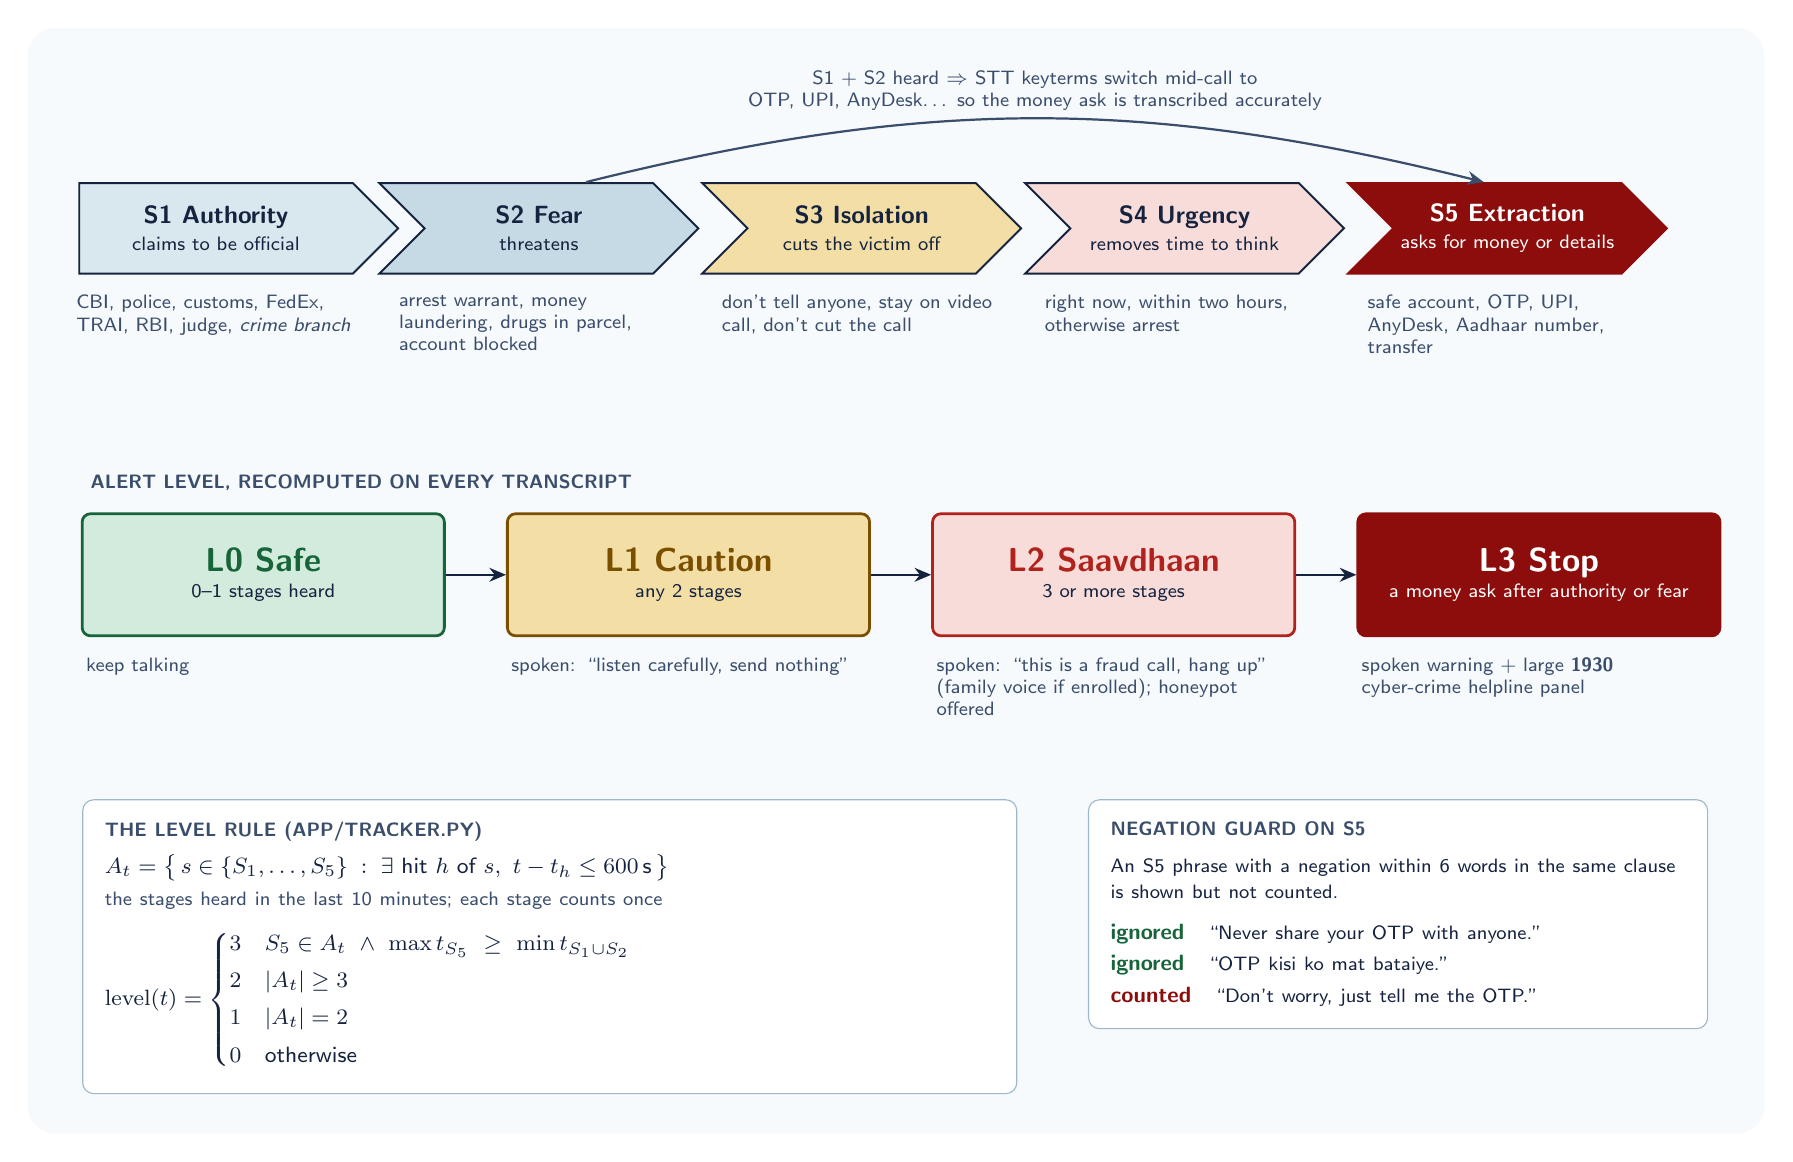
\begin{tikzpicture}[x=1cm,y=1cm,
  chev/.style={signal, signal to=east, signal from=west, draw=ink, line width=0.7pt,
               minimum width=4.05cm, minimum height=1.15cm, align=center, inner sep=2pt},
  ex/.style={text width=3.55cm, align=left, execute at begin node={\hyphenpenalty=10000\exhyphenpenalty=10000}, font=\scriptsize, text=inksoft},
  lvl/.style={rounded corners=3pt, line width=1pt, minimum width=4.6cm, minimum height=1.55cm,
              align=center, inner sep=4pt}]

% ---- the five stages --------------------------------------------------------------
\node[chev, signal from=nowhere, fill=paper]     (s1) at (2.0,6) {\modtitle{S1 Authority}\\{\scriptsize claims to be official}};
\node[chev, fill=paperdeep]                      (s2) at (6.1,6) {\modtitle{S2 Fear}\\{\scriptsize threatens}};
\node[chev, fill=cautionwash]                    (s3) at (10.2,6) {\modtitle{S3 Isolation}\\{\scriptsize cuts the victim off}};
\node[chev, fill=dangerwash]                     (s4) at (14.3,6) {\modtitle{S4 Urgency}\\{\scriptsize removes time to think}};
\node[chev, fill=stop, text=white, draw=stop]    (s5) at (18.4,6) {\modtitle{\color{white}S5 Extraction}\\{\scriptsize\color{white} asks for money or details}};

\node[ex, below=4pt of s1] {CBI, police, customs, FedEx, TRAI, RBI, judge, \emph{crime branch}};
\node[ex, below=4pt of s2] {arrest warrant, money laundering, drugs in parcel, account blocked};
\node[ex, below=4pt of s3] {don't tell anyone, stay on video call, don't cut the call};
\node[ex, below=4pt of s4] {right now, within two hours, otherwise arrest};
\node[ex, below=4pt of s5] {safe account, OTP, UPI, AnyDesk, Aadhaar number, transfer};

% stage-following keyterms
\draw[flow, draw=inksoft] ($(s2.north)+(0.6,0)$) to[bend left=14]
  node[lab, above=1pt, align=center] {S1 + S2 heard $\Rightarrow$ STT keyterms switch mid-call to\\ OTP, UPI, AnyDesk\ldots\ so the money ask is transcribed accurately}
  ($(s5.north)+(-0.3,0)$);

% ---- alert levels -----------------------------------------------------------------
\node[lvl, draw=safe, fill=safewash]       (l0) at (2.6,1.6)  {{\large\bfseries\color{safe} L0 Safe}\\{\scriptsize 0--1 stages heard}};
\node[lvl, draw=caution, fill=cautionwash] (l1) at (8.0,1.6)  {{\large\bfseries\color{caution} L1 Caution}\\{\scriptsize any 2 stages}};
\node[lvl, draw=danger, fill=dangerwash]   (l2) at (13.4,1.6) {{\large\bfseries\color{danger} L2 Saavdhaan}\\{\scriptsize 3 or more stages}};
\node[lvl, draw=stop, fill=stop, text=white] (l3) at (18.8,1.6) {{\large\bfseries\color{white} L3 Stop}\\{\scriptsize\color{white} a money ask after authority or fear}};
\foreach \a/\b in {l0/l1, l1/l2, l2/l3} \draw[flow] (\a) -- (\b);
\node[anchor=south west] at ($(l0.north west)+(0,0.15)$) {\grouptag{Alert level, recomputed on every transcript}};

\node[ex, text width=4.5cm, below=4pt of l0] {keep talking};
\node[ex, text width=4.5cm, below=4pt of l1] {spoken: ``listen carefully, send nothing''};
\node[ex, text width=4.5cm, below=4pt of l2] {spoken: ``this is a fraud call, hang up'' (family voice if enrolled); honeypot offered};
\node[ex, text width=4.5cm, below=4pt of l3] {spoken warning + large \textbf{1930} cyber-crime helpline panel};

% ---- the rule, in maths --------------------------------------------------------------
\node[draw=rule, fill=white, rounded corners=4pt, inner sep=8pt, anchor=north west, text width=11.3cm] (rule) at (0.3,-1.25) {%
  \grouptag{The level rule (app/tracker.py)}\\[4pt]
  $A_t=\bigl\{\,s\in\{S_1,\dots,S_5\} \;:\; \exists\ \text{hit } h \text{ of } s,\ t-t_h\le 600\,\text{s}\,\bigr\}$
  \\[2pt]{\scriptsize\color{inksoft} the stages heard in the last 10 minutes; each stage counts once}\\[6pt]
  $\displaystyle \operatorname{level}(t)=
  \begin{cases}
    3 & S_5\in A_t \ \wedge\ \max t_{S_5} \ \ge\ \min t_{S_1\cup S_2}\\[2pt]
    2 & |A_t|\ge 3\\[2pt]
    1 & |A_t| = 2\\[2pt]
    0 & \text{otherwise}
  \end{cases}$};

% ---- negation guard -------------------------------------------------------------------
\node[draw=rule, fill=white, rounded corners=4pt, inner sep=8pt, anchor=north east, text width=7.3cm] (neg) at (20.95,-1.25) {%
  \grouptag{Negation guard on S5}\\[4pt]
  {\scriptsize An S5 phrase with a negation within 6 words in the same clause is shown but not counted.}\\[5pt]
  \textbf{\color{safe}ignored}\quad {\scriptsize ``Never share your OTP with anyone.''}\\[2pt]
  \textbf{\color{safe}ignored}\quad {\scriptsize ``OTP kisi ko mat bataiye.''}\\[2pt]
  \textbf{\color{stop}counted}\quad {\scriptsize ``Don't worry, just tell me the OTP.''}};

\card
\end{tikzpicture}
\end{document}
